% ОБЯЗАТЕЛЬНО ИМЕННО ТАКОЙ documentclass!
% (Основной кегль = 14pt, поэтому необходим extsizes)
% Формат, разумеется, А4
% article потому что стандарт не подразумевает разделов
% Глава = section, Параграф = subsection
% (понятия "глава" и "параграф" из документа, описывающего диплом)
\documentclass[a4paper,article,14pt]{extarticle}

% Подключаем главный пакет со всем необходимым
\usepackage{spbudiploma_tempora}

% Пакеты по желанию (самые распространенные)
% Хитрые мат. символы
\usepackage{euscript}
% Таблицы
\usepackage{longtable}
\usepackage{makecell}
% Картинки (можно встявлять даже pdf)
\usepackage[pdftex]{graphicx}

\usepackage{amsthm,amssymb, amsmath}
\usepackage{textcomp}

\begin{document}

% Титульник в файле titlepage.tex
% --------------------- Титульник ВКР СПбГУ -----------------------------
% Автор: Тоскин Николай, itonik@me.com
% Если заметили ошибку, напишите на email
% Если хотите добавить изменение самостоятельно:
% https://github.com/itonik/spbu_diploma/
% Использованы материалы:
% habr.com/ru/post/144648/
% cpsconf.ru
% Документы ниже могут уже быть неактуальны, тем не менее за годы ничего
% нового не появилось
% Текст:
% http://edu.spbu.ru/images/data/normativ_acts/local/20181030_10432_1.pdf
% Титульный лист:
% http://edu.spbu.ru/images/data/normativ_acts/local/20180703_6616_1.pdf
% -----------------------------------------------------------------------

% Титульный лист диплома СПбГУ
% Временное удаление foot на titlepage
\newgeometry{left=30mm, top=20mm, right=15mm, bottom=20mm, nohead, nofoot}
\begin{titlepage}
\begin{center}

\textbf{Санкт--Петербургский}
\textbf{государственный университет}

\vspace{35mm}

\textbf{\textit{\large ЦАРЁВ Никита Евгеньевич}} \\[8mm]
% Название
\textbf{\large Выпускная квалификационная работа}\\[3mm]
\textbf{\textit{\large Разработка обучающего веб-инструмента удаленной сборки и интерактивной отладки программ}}

\vspace{20mm}
Уровень образования: бакалавриат\\
Направление 01.03.02 «Прикладная математика и информатика»\\
Основная образовательная программа СВ.5005.2018
«Прикладная математика, фундаментальная информатика и программирование»\\
Профиль «Современное программирование»\\[15mm]


% Научный руководитель, рецензент
\begin{flushright}
\begin{minipage}[t]{0.65\textwidth}
{Научный руководитель:} \\
профессор, факультет математики и компьютерных наук Санкт--Петербургского
государственного университета, д.ф. - м.н. Куликов~Александр Сергеевич

\vspace{10mm}

{Рецензент:} \\
доцент Новгородского государственного университета имени Ярослава Мудрого,
к. т. н. Довгалюк~Павел Михайлович
\end{minipage}
\end{flushright}

\vfill

{Санкт-Петербург}
\par{\the\year{} г.}
\end{center}
\end{titlepage}
% Возвращаем настройки geometry обратно (то, что объявлено в преамбуле)
\restoregeometry
% Добавляем 1 к счетчику страниц ПОСЛЕ titlepage, чтобы исключить
% влияние titlepage environment
\addtocounter{page}{1}


% Содержание
\tableofcontents
\pagebreak

\specialsection{Введение}

В настоящее время обучение языку ассемблера является важной составляющей многих программистских курсов.

Очень часто студенты, изучающие язык ассемблера, сталкиваются с проблемами при настройки среды разработки, при использовании инструментов компиляции и отладки.

Преподаватели таких курсов также сталкиваются с проблемами организации учебного процесса.

Создание удобного, интерактивного и производительного программного инструмента удалённой сборки и отладки програм на ассемблере, представляет собой актуальную задачу.

\specialsection{Постановка задачи}

\textbf{Цель данной работы} состоит в разработке обучающего веб-инструмента удалённого запуска, отладки и проверки программ на языке ассемблера.

\textbf{Задачи данной работы}:

\begin{enumerate}
    \item Исследование существующих решений для запуска и отладки программ на языке ассемблера, а также решений для обучения языку ассемблера.
    \item Формирование требований к разрабатываемому инструменту.
    \item Исследование возможности создания инструмента.
    \item Разработка программной архитектуры инструмента.
    \item Реализация инструмента.
    \item Исследование свойств решения.
\end{enumerate}

\textbf{Объектом исследования} являются системы запуска и отладки программ на языке ассемблера.

\textbf{Предметом исследования} является интерактивность и удобство использования таких систем.

\textbf{Практическая ценность работы} состоит в том, что разработанный инструмент позволит проводить обучение языку ассемблера более эффективно для студентов.

\section{Обзор предметной области}
\subsection{Критерии сравнения}

В мире существует множество решений для запуска ассемблерного кода, а также решений для обучения языку ассемблера. В этой главе рассматривается несколько таких решений, каждое из них анализируется в контексте следующих \textbf{критериев сравнения}:

\begin{enumerate}
    \item Поддержка запуска ассемблерного кода на разных диалектах и на разных архитектурах.
    \item Поддержка отладки: выполнение по шагам, поддержка точек останова, редактирования регистров/памяти, визуализация стека вызовов.
    \item Поддержка задач и их автоматической проверки.
    \item Поддержка интеграции с системами управления обучением.
    \item Возможность работы без установки дополнительного программного обеспечения на устройстве пользователя.
    \item Возможность самостоятельной установки и развёртывания системы на выделенном сервере, доступность исходного кода.
\end{enumerate}

\subsection{Существующие решения}
\subsubsection{Ideone}

Ideone\footnote{\url{https://ideone.com}} является онлайн компилятором и средой разработки, поддерживающей более 60 языков программирования, в том числе несколько диалектов ассемблера.

Поддерживается запуск ассемблерного кода на архитектурах x86 (NASM и GNU диалекты) и x86-64 (только NASM диалект). Отладка не поддерживается.

Поддержки задач, их автоматической проверки нет, соответственно нет и интеграции в системы управления обучением.

Взаимодействие с системой происходит через веб-интерфейс, установки допольнительного ПО не требуется.

Система имеет закрытый исходный код, самостоятельно установить систему на выделенный сервер не представляется возможным.

\subsubsection{OneCompiler}

OneCompiler\footnote{\url{https://onecompiler.com/assembly}} является онлайн компилятором и средой разработки, поддерживающей, в том числе, и NASM диалект x86 ассемблера.

Поддержиывается запуск кода, есть возможность указать содержимое стандартного потока ввода перед запуском. Отладка не поддерживается.

Поддержки задач, их автоматической проверки нет, соответственно нет и интеграции в системы управления обучением.

Взаимодействие с системой происходит через веб-интерфейс, установки допольнительного ПО не требуется.

Система имеет закрытый исходный код, самостоятельно установить систему на выделенный сервер не представляется возможным.

\subsubsection{ASM Debugger}

ASM Debugger\footnote{\url{http://asmdebugger.com}} является инструментом для пошаговой отладки простых программ на языке ассемблера.

Особенностью инструмента является то, что он не использует запуск программ на реальном аппаратном обеспечении. Вместо этого, на языке Javascript реализовано подмножество инструкций x86 ассемблера.

Поддерживается запуск ассемблерного кода на архитектуре x86 с NASM диалектом. Поддерживается пошаговое исполнение, просмотр значений регистров.

Поддержки задач, их автоматической проверки нет, соответственно нет и интеграции в системы управления обучением.

Взаимодействие с инструменетом происходит через веб-интерфейс, установки допольнительного ПО не требуется.

Инструмент имеет открытый исходный код\footnote{\url{https://github.com/dinoqqq/asmdebugger}}, соответственно есть возможность установить его на выделенный сервер.

\subsubsection{SASM (SimpleASM)}

SASM\footnote{\url{https://dman95.github.io/SASM/index.html}} представляет из себя кроссплатформенную среду разработки на языке ассемблера для архитектур x86 и x86-64 с использованием диалектов NASM, GNU, FASM, MASM.

Поддерживается запуск ассемблерного кода, поддерживается выполнение по шагам, точки останова, просмотр и редактирование регистров и памяти, а также произвольные команды GDB.

Поддержки задач, их автоматической проверки нет, соответственно нет и интеграции в системы управления обучением.

Для использования инструмента необходима его установка на компьютер пользователя. Инструмент имеет открытый исходный код\footnote{\url{https://github.com/Dman95/SASM}}.

\subsubsection{JetBrains Clion + EduTools}

Clion\footnote{\url{https://www.jetbrains.com/clion/}}~--- это интегрированная среда разработки от компании JetBrains, предназначенная, в первую очередь, для разработки приложений на языках C и C++. Язык ассемблера не поддерживается ни в каком виде, но существуют сторонние плагины, которые решают эту проблему, например NASM Assembly Language\footnote{\url{https://plugins.jetbrains.com/plugin/9759-nasm-assembly-language}}.

Компиляция и запуск кода на языке ассемблера возможны, если модифицировать должным образом файлы системы описания сборки CMake. Отладка ассемблерного кода не поддерживается.

Плагин EduTools\footnote{\url{https://plugins.jetbrains.com/plugin/10081-edutools}} позволяет создавать и писать задачи с автоматическими тестами, что упрощает проверку решений. Отсутствует поддержка задач с закрытыми (недоступными для обучающегося) тестами. Интеграция с системами управления обучением отсутствует.

Для использования данной среды разработки необходима её установка на компьютер пользователя. Она имеет закрытый исходный код.

\subsubsection{GitHub Classroom + Visual Studio Code}

GitHub Classroom~--- это сервис, позволяющий давать учебные задания в виде git-репозиториев. GitHub Classroom позволяет добавить кнопку <<открыть в Visual Studio Code>>, которая позволяет открыть репозиторий с преднастроенными плагинами в этом редакторе.

Для того, чтобы настроить поддержку языка ассемблера в Visual Studio Code, требуется установка дополнительных плагинов. Также преподавателю в шаблонном репозитории необходимо будет настроить компиляцию и запуск в файлах \texttt{tasks.json} и \texttt{launch.json}. Отладка не поддерживается.

GitHub Classroom позволяет добавлять тесты через веб-интерфейс преподавателя. В качестве теста может выступать набор входных данных и эталонных ответов к ним, так и путь до скрипта для автоматической проверки. В первом случае входные данные передаются программе через стандартный поток ввода, а вывод программы сравнивается с эталонным ответом.

Необходима установка Visual Studio Code, компилятора и отладчика.

GitHub Classroom имеет закрытый исходный код, установить свою копию на выделенный сервер не представляется возможным.

\subsubsection{Stepik}

В системе управления обучением Stepik\footnote{\url{https://stepik.org}} есть режим задания Code Challenge, который позволяет проверять код, написанный на различных языках программирования.

Поддерживается NASM диалект x86 и x86-64 ассемблера. Отладка не поддерживается.

Поддерживаются задачи и их автоматическая проверка на скрытых тестах. Тесты должны иметь вид набора входных данных и эталонных ответов. Входные данные передаются программе через стандартный поток ввода, а вывод программы сравнивается с эталонным ответом.

Взаимодействие с системой происходит через веб-интерфейс, установка дополнительного ПО не требуется. Система имеет закрытый исходный код.

\subsubsection{Moodle + Virtual Programming Lab}

Для системы управления обучением Moodle\footnote{\url{https://moodle.org/}} существует плагин Virtual Programming Lab\footnote{\url{https://vpl.dis.ulpgc.es}}, котторый позволяет запускать и проверять код, написанный на различных языках программирования.

Поддерживается NASM диалект x86 ассемблера, отладка не поддерживается.

Поддерживаются задачи и их автоматическая проверка на скрытых тестах. Тесты должны иметь вид набора входных данных и эталонных ответов. Входные данные передаются программе через стандартный поток ввода, а вывод программы сравнивается с эталонным ответом.

Взаимодействие с системой происходит через веб-интерфейс, установка дополнительного ПО не требуется. И система Moodle и плагин Virtual Programming Lab имеют открытый исходный код. Соответственно, есть возможность установки этой связки на выделенный сервер.

\subsubsection{Git репозиторий с заданиями и скриптами для проверки}

Одним из популярных способов организовать проверку заданий при проведении курсов по программированию является специально организованный git репозиторий. К примеру может ожидаться, что студенты выполняют задания в своих локальных копиях, а задания проверяются специально написанными скриптами, расположенными в том же репозитории.

При таком подходе, учащиеся могут выбирать любой удобный им редактор кода. Для запуска кода могут быть предоставлены готовые скрипты. То же самое нельзя сказать об отладке, скорее всего студенту придётся познакомиться с gdb или другой подобной утилитой.

Такой подход применяется в учебном процессе на практике. Возможно автоматизировать и генерацию репозиториев с задачами для каждого пользователя, и закрытые тесты, и даже интеграцию с системами управления обучением. На практике таким мало кто занимается.

Такой подход требует от орагнизаторов курса реализовать скрипты запуска и проверки решений. От студентов же требуется установка дополнительного программного обеспечения (такого как git, компилятор, отладчик) и наличие навыков работы с инструментами командной строки. Также может требоваться использование конкретной операционной системы, так как зачастую скрипты расчитывают на наличие конкретного пользовательского окружения.


\subsection{Сравнение существующих решений}

Краткая информация о решениях представлена в таблице \ref{table:alternatives}.

\begin{center}
\small
    \begin{longtable}{|p{3.5cm}|p{2cm}|p{2cm}|p{2cm}|p{2cm}|p{2cm}|}
    \caption{Сравнение существующих решений}\label{table:alternatives} \\
    \hline
    \textbf{Решение} & \textbf{Диалект} & \textbf{Отладка} & \textbf{Учебный процесс} & \textbf{Нужна установка} & \textbf{Открытый исходный код} \\
    \hline
    Ideone & x86 (NASM, GNU), x86\_64 (NASM) & нет & нет & нет & нет \\ \hline
    OneCompiler & x86 NASM & нет & нет & нет & нет \\ \hline
    ASM Debugger & x86 NASM (подмножество) & да\footnote{Поддерживается пошаговое исполнение, просмотр значений регистров} & нет & нет & да \\ \hline
    SASM & x86, x86\_64 (NASM, GNU, FASM, MASM) & да & нет & да & да \\ \hline
    Clion + EduTools & x86 NASM\footnote{Только со сторонним плагином} & нет & частично\footnote{Задачи поддерживаются, интеграции с системами управления обучением нет} & да & нет \\ \hline
    GitHub + VSCode & зависит от настроек & нет & частично & да & нет \\ \hline
    Stepik & x86, x86\_64 NASM & нет & да & нет & нет \\ \hline
    Moodle + VPL & x86 NASM & нет & да & нет & да \\ \hline
    Git репозиторий & зависит & нет & частично & да & --- \\ \hline
    \end{longtable}
\normalsize
\end{center}

Среди расмотренных альтернатив можно выделить несколько групп схожих решений.

Первой такой группой являются онлайн компиляторы. К ним можно отнести Ideone и OneCompiler. Они представляют веб редакторы с возможностью компиляции и запуска кода на разных языках. В этих системах языку ассемблера не уделяется особого внимания, так как основная масса пользователей таких систем использует их для написания кода на высокоуровневых языках. Также эти системы имеют закрытый исходный код.

В качестве второй группы можно выделить такие системы как Stepik, Moodle и JetBrains EduTools. Они предназначены, в первую очередь, для образовательных процессов. Поддержка задач, направленных на иизучение языка ассемблера, не является их основной целью. Так, для системы Moodle, требуется сторонний плагин, а среды разработки JetBrains поддерживают механизм отладки многих языков программирования, но не ассемблера.

Также хочется выделить решения, требующие сложной настройки со стороны преподавателей, такие как интеграция GitHub Classroom с Visual Studio Code и использование git репозитория для организации учебного процесса. Эти решения отличаются гибкостью, но требуют написания скриптов и конфигурационных файлов перед использованием. Также они требуют установки дополнительного программного обеспечения на компьютерах студентов.

В качестве последней категории можно выделить средства, предназначенные именно для запуска и отладки ассемблерного кода, но не поддерживающие интеграцию в учебный процесс, такие как ASM Debugger и SASM. Так как эти инструменты направлены именно на работу с языком ассемблера, они обладают большим функционалом по сравнению с другими, более общими решениями. Например, они поддерживают отладку программ на ассемблере, чего не поддерживает ни одна другая рассмотренная альтернатива.

\subsection{Выводы}

В этой главе были рассмотрены различные решения для запуска и отладки программ на языке ассемблера, а также решения, предназначенные для обучения языку ассемблера. Исходя из обзора предметной области, можно сделать вывод, что имеется недостаток решений, одновременно позволяющих производить отладку программ на языке ассемблера, интегрироваться в учебный процесс и не требовать установки и настройки на устройстве пользователя.

\section{Формулировка требований к решению}

\subsection{Функциональные требования}

Наиболее важными характеристиками разрабатываемого инструмента будут те, которые выгодно его отличают от существующих аналогов. Исходя из этого, были сформулированы следующие функциональные требования к инструменту:

\begin{enumerate}
    \item Инструмент должен быть доступен через веб-интерфейс и не требовать установки допольнительного программного обеспечения на устройстве пользователя.
    \item Инструмент должен содержать возможность аутентификации пользователей, как по паре логин/пароль, так и через протокол LTI.
    \item Должна существовать возможность разделения прав пользователей на администраторов и учащихся.
    \item Администраторы должны иметь возможность создавать, редактировать и удалять задачи.
    \item Каждая задача должна иметь: название, текст условия, связанный с ней чекер и его параметры.
    \item Учащиеся должны уметь получать задания по конкретным задачам через системы управления обучением. Для этого администратор такой системы должен настроить LTI интеграцию, в частности, указать идентификатор нужной задачи.
    \item На странице задания для учащегося должно быть доступно условие задачи, редактор кода, возможность отправить решение на проверку и информация о предыдущих попытках решения.
    \item Вместе с редактором кода должна быть доступна функциональность отладки: добавление и удаление точек останова, запуск, остановка, пошаговое исполнение программы. Если программа находится в приостановленном состоянии, должен быть доступен просмотр и редактирование регистров процессора и содержимого памяти процесса. Должна поддерживаться архитектура x86\_64.
    \item Запускаемые пользовательские программы должны быть ограничены по времени и используемой памяти, им должен быть запрещен доступ к файловой системе, сети, процессам и другим ресурсам операционной системы.
\end{enumerate}

\subsection{Нефункциональные требования}

\begin{enumerate}
    \item Инструмент, в первую очередь, предназначается для задач, направленных непосредственно на изучение языка ассемблера. Таким образом, задачи должны быть составлены так, чтобы их решения могли исполняться в контексте непривилегированных процессов пользовательского пространства, без доступа к конкретным системным вызовам и периферии.
    \item Инструмент должен минимизировать количество элементарных шагов, требуемых для запуска программ.
    \item Инструмент должен быть эффективен по использованию процессорного времени и оперативной памяти.
    \item Инструмент должен обладать достаточным быстродействием и отзывчивостью.
\end{enumerate}

\section{Архитектура программной реализации}

\subsection{Структура программной реализации}

Реализация инструмента представляет из себя несколько сервисов, общающихся между собой по различным протоколам. Схема взаимодействия процессов в системе представлена на рисунке \ref{fig:processes_arch}.

\begin{figure}[ht]
    \begin{center}
        \scalebox{0.8}{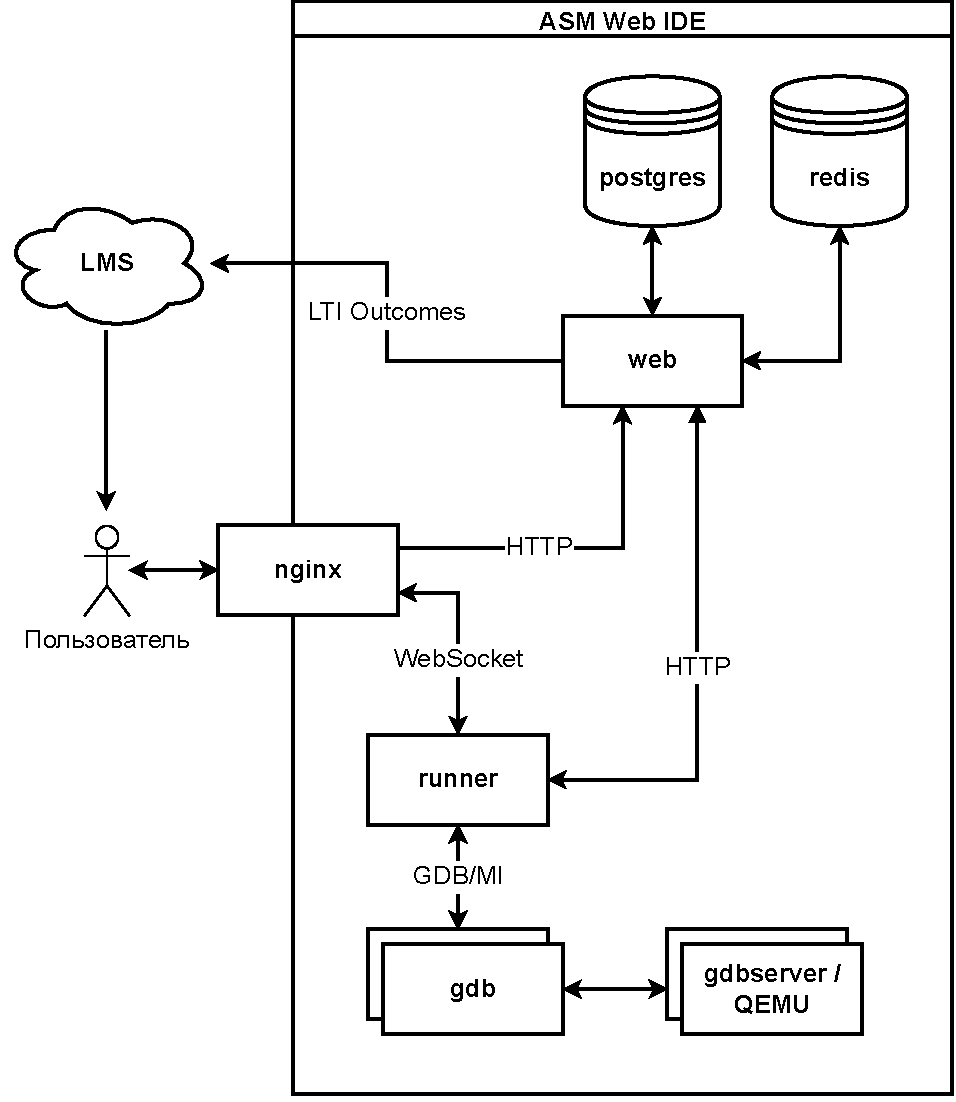
\includegraphics{images/processes_arch.pdf}}
        \caption{\label{fig:processes_arch} Схема взаимодействия процессов в системе}
    \end{center}
\end{figure}

Сервис \textbf{web} представляет из себя приложение, написанное на языке Python с использованием фреймворка Flask. Он отвечает за основную бизнес-логику инструмента. Сервис предоставляет функционал аутентификации и авторизации, как через протокол LTI, так и по паре логин/пароль. Для студентов сервис предоставляет интерфейс просмотра задач и решений, а для преподавателей~--- панель управления, позволяющую создавать и редактировать задачи, просматривать попытки решения и информацию о пользователях.

Сервис \textbf{runner} представляет из себя приложение, написанное на языке Python с использованием библиотеки AIOHTTP. Он отвечает за управление сессиями отладки, взаимодействие с процессами отладчика через протокол GDB/MI, а также за взаимодействие с пользователями через протокол WebSocket. Помимо предоставления возможности интерактивной отладки веб-интерфейсу, этот сервис также занимается автоматизированной проверкой решений. Эта функциональность недоступна для внешнего пользователя напрямую, запросы на проверку решений отправляет сервис web по протоколу HTTP.

Базы данных \textbf{postgres} и \textbf{redis} используются для хранения необходимой для работы системы информации. В PostgreSQL хранится информация о пользователях, задачах, заданиях и посылках. Также там хранится метаинформация об интерактивных сессиях отладки. В Redis хранится множество использованных значений nonce при авторизации систем управления обучением по протоколу LTI.

Система мониторинга \textbf{prometheus} предоставляет интерфейс для просмотра различных метрик, описывающих состояние системы. Метрики собираются как и с самого Prometheus, так и с сервиса runner через протокол HTTP.

Веб-сервер \textbf{nginx} используется в качестве обратного прокси-сервера, проксирующего HTTP запросы в сервис web и взаимодействие по протоколу WebSocket с сервисом runner. Также Nginx отдаёт статические файлы и проксирует сервис мониторинга Prometheus. Перед доступом к Prometheus, Nginx подтверждает у web наличие у пользователя прав администратора.

\subsection{Компиляция ассемблерных программ}

Используем GCC. Поддерживаются директивы \texttt{\#line}, таким образом можно чинить номера строк с отладочной информации и сообщениях об ошибках.

\subsection{Запуск ассемблерных программ}

\subsubsection{Изоляция с помощью seccomp}

Seccomp~--- механизм ядра Linux, позволяющий процессу перейти в <<безопасный режим>>, в котором запрещены все системные вызовы, кроме \texttt{exit}, \texttt{sigreturn}, \texttt{read} и \texttt{write}. Запретить работать со стандартными потоками ввода/вывода можно, предварительно вызвав \texttt{close} на них.

Здесь можно привести листинг кода, который переводит программу в безопасный режим. Код этот живёт в файле \texttt{environment/x86\_64/entry.S}.

\subsubsection{Ограничение потребляемых ресурсов с помощью Docker}

Docker (через механизм контрольных групп) позволяет ограничивать использование процессорного времени, используемую память в контейнерах.

Существует системный вызов \texttt{setrlimit}. Ограничиваем процессорное время в секундах через \texttt{RLIM\_CPU}. Docker умеет это делать через параметр \texttt{ulimit}.

\subsection{Отладка ассемблерных программ}

\subsubsection{Использование GDB}

GDB~--- консольный инструмент отладки программ. Позволяет отлаживать программы на самых разных языках программирования на разных платформах. Поддерживает отладочную информацию в формате DWARF.

\subsubsection{GDB/MI}

GDB/MI (GDB Machine Interface, машинный интерфейс GDB) позволяет взаимодействовать с процессом отладки в машиночитаемом виде. Это нам пригодится.

Тут можно вкратце описать формат взаимодействия, сослаться на мануал GDB/MI.

\subsubsection{GDB server}

GDB server~--- программа, с которой GDB может взаимодействовать, чтобы организовать отладку кода на удалённой машине. Пригодится для разделения полномочий и ограничения ресурсов.

\subsection{Взаимодействие с пользователем через веб-браузер}

Для интерактивной отладки необходимо не только передавать команды из веб-интерфейса в GDB, но и асинхронно реагировать на события, возникающие при отладки. К таким событиям, например, относится остановка программы на точке останова. К счастью, все современные браузеры поддерживают протокол WebSocket, который позволяет общаться клиенту и серверу полностью асинхронно, а не по модели запрос-ответ.

\subsection{Взаимодействие с системами управления обучением}

Существует такой протокол: LTI, Learning Tools Interoperability. В частности, позволяет по протоколу OAuth авторизовывать пользователей конкретной LMS, получать информацию о таске, а также отправлять результаты проверки как score от 0.0 до 1.0.

\subsection{Сбор метрик}

Поднимаем Prometheus, пишем туда нужные метрики. Идеи для релевантных метрик: задержка исполнения команд gdb, время реакции на команды пользователя, общее потребление памяти на процесс отладки (gdb + gdbserver + программа), потребление cpu на процесс отладки (интересует idle cpu usage).

\subsection{Интерфейс пользователя}

\subsubsection{Аутентификация через логин и пароль}

Есть у нас страница \texttt{/login}. Ожидается, что так входят только админы.

\subsubsection{Аутентификация через LTI}

При правильно настроенном Moodle, достаточно зайти на страницу задания и увидеть iframe с интерфейсом пользователя, вход происходит автоматически. Под капотом нам POST запрос к ручке \texttt{/lti} с нужными параметрами.

Скриншот мудла с iframeом.

\subsubsection{Работа с интерактивным отладчиком через GUI}

Можно ставить брейкпоинты, можно слать команды, можно смотреть на регистры. Обратите вниманеи на красивый редактор. Скриншот в paused состоянии.

\subsubsection{Работа с админской панелью}

Есть несколько сущностей: пользователи, задачи, задания и посылки, с ними работа ведётся одинаково.

\subsection{Модель данных}

\subsubsection{Схема базы данных}

Тут схема, которую как-то надо нарисовать.

\subsubsection{Таблица users}

Содержит в себе данные о пользователях, в том числе и метод аутентификации (password или LTI).

\subsubsection{Таблица problems}

Содержит информацию о задачах, в том числе и чекер.

\subsubsection{Таблица assignments}

Задания, выданные студентам. Содержит, помимо прочего, LTI callback и оценку.

\subsubsection{Таблица submissions}

Содержит посылки по задачам.

\section{Исследование свойств решения}

\specialsection{Выводы}

Ну вот написали инструмент, все задачи поставленные во введении сделали.

% Библиография в cpsconf стиле
% Аргумент {1} ниже включает переопределенный стиль с выравниванием слева
\begin{thebibliography}{1}
% \bibitem{voc} Griffin D.W., Lim J.S. \flqq Multiband excitation vocoder\frqq. IEEE ASSP-36 (8), 1988, pp. 1223-1235.
% \bibitem{vo2} Griffin D.W., Lim J.S. \flqq Multiband excitation vocoder\frqq. IEEE ASSP-36 (8), 1988, pp. 1223-1235.
\end{thebibliography}
\end{document}
